% vtc2026_paper.tex — IEEE VTC2026-Fall Submission
% Target: 5 pages (up to 7 with extra charge), double-blind
\documentclass[conference]{IEEEtran}

% ────────── packages ──────────
\usepackage[T1]{fontenc}
\usepackage[utf8]{inputenc}
\usepackage{amsmath,amssymb}
\usepackage{graphicx}
\usepackage{booktabs}
\usepackage{multirow}
\usepackage{array}
\usepackage{tabularx}
\usepackage{siunitx}
\usepackage{xcolor}
\usepackage{tikz}
\usetikzlibrary{positioning, decorations.pathreplacing, calc}
\usepackage{pgfplots}
\usepackage{pgfplotstable}
\usepackage{url}
\usepackage[hidelinks]{hyperref}
\usepackage{cite}
\usepackage{balance}
\usepackage{colortbl}
\usepackage{enumitem}
\pgfplotsset{compat=1.18}

% ────────── compact spacing ──────────
\setlist{nosep,leftmargin=*}
\renewcommand{\arraystretch}{1.05}

% ────────── custom commands ──────────
\newcommand{\sysname}{\textsc{PQ\nobreakdash-Tunnel}}
\newcommand{\us}{\,\si{\micro\second}}
\newcommand{\ms}{\,\si{\milli\second}}
\newcommand{\mW}{\,\si{\milli\watt}}
\newcommand{\uJ}{\,\si{\micro\joule}}
\newcommand{\mJ}{\,\si{\milli\joule}}
\newcommand{\MBs}{\,\si{MB/s}}
\newcommand{\eg}{\textit{e.g.}}
\newcommand{\ie}{\textit{i.e.}}
\newcommand{\etal}{\textit{et al.}}

% ────────── level colors ──────────
\definecolor{lvlone}{HTML}{E8F5E9}
\definecolor{lvlthree}{HTML}{FFF3E0}
\definecolor{lvlfive}{HTML}{FFEBEE}
\definecolor{bestcell}{HTML}{C8E6C9}
\definecolor{worstcell}{HTML}{FFCDD2}

% ────────── double-blind: comment out for camera-ready ──────────
% \author{
%   \IEEEauthorblockN{Author Names Omitted for Double-Blind Review}
%   \IEEEauthorblockA{Affiliation Omitted}
% }

\begin{document}

\title{Post-Quantum Cryptographic Overhead on Embedded UAV\\Hardware: A Measurement-Driven Analysis}

\author{\IEEEauthorblockN{Paper ID: XXXX — Submitted for Double-Blind Review}}

\maketitle

% ═══════════════════════════════════════════════════════════════
%  ABSTRACT
% ═══════════════════════════════════════════════════════════════
\begin{abstract}
Unmanned aerial vehicles rely on the MAVLink protocol, which transmits
telemetry and commands in plaintext.  As quantum computers advance
toward cryptographic relevance, classical key exchange and signatures
face obsolescence.  We deploy a transparent post-quantum cryptographic
proxy on a Raspberry~Pi~4 (Cortex-A72, 1.8\,GHz) that protects
MAVLink traffic without modifying the autopilot firmware.  Using an
INA219 current sensor sampling at 1\,kHz, we measure execution time,
power draw, and energy consumption for nine key encapsulation
mechanisms, eight digital signature schemes, and three authenticated
encryption ciphers across all NIST security levels (1, 3, 5).
The 24 level-matched KEM--signature pairs compose 72 cipher suites
whose handshake cost spans four orders of magnitude, from 11\,ms
(ML-KEM-512\,+\,Falcon-512) to over 9\,s (McEliece-8192128\,+\,SPHINCS\textsuperscript{+}-256s).
We further quantify the overhead of on-board DDoS detection, showing
that an XGBoost sentinel adds 951\,mW while a Transformer model
doubles CPU utilisation to 93\%.  These measurements feed a graceful-degradation
scheduler that selects cipher suites at runtime to satisfy
energy and thermal constraints on battery-powered aircraft.
\end{abstract}

\begin{IEEEkeywords}
Post-quantum cryptography, UAV security, MAVLink, embedded benchmarks,
power measurement, cipher suite selection, DDoS detection
\end{IEEEkeywords}

% ═══════════════════════════════════════════════════════════════
%  I.  INTRODUCTION
% ═══════════════════════════════════════════════════════════════
\section{Introduction}
\label{sec:intro}

Small unmanned aerial vehicles have become indispensable in
agriculture, infrastructure inspection, and emergency response.
Most open-source autopilots communicate with ground control stations
through the MAVLink protocol~\cite{mavlink-spec}, a lightweight
binary format designed for bandwidth-constrained radio links.
MAVLink version~2 offers an optional 48-bit signature for integrity,
yet it provides no encryption: every heartbeat, GPS coordinate, and
actuator command travels in cleartext.

The arrival of large-scale quantum computers will render RSA and
elliptic-curve key exchange vulnerable to Shor's algorithm~\cite{shor1994}.
An adversary who records encrypted traffic today can decrypt it once
a sufficiently powerful quantum machine becomes available, a strategy
known as \emph{harvest-now, decrypt-later}.  For drone operations
involving critical infrastructure or military reconnaissance, a
ten-year shelf life on captured telemetry is well within plausible
threat horizons.

NIST concluded its Post-Quantum Cryptography standardisation in 2024,
publishing ML-KEM (FIPS~203)~\cite{nist-fips203} for key encapsulation,
ML-DSA (FIPS~204)~\cite{nist-fips204} for digital signatures, and
SLH-DSA (FIPS~205)~\cite{nist-fips205} as a conservative hash-based
alternative.  Fourth-round candidates HQC~\cite{hqc} and
Classic~McEliece~\cite{mceliece} remain under evaluation.
While desktop and server benchmarks of these algorithms abound, the
embedded ARM ecosystem that dominates drone companion computers
has received far less attention.

\begin{figure}[b]
  \centering
  \resizebox{\columnwidth}{!}{%
  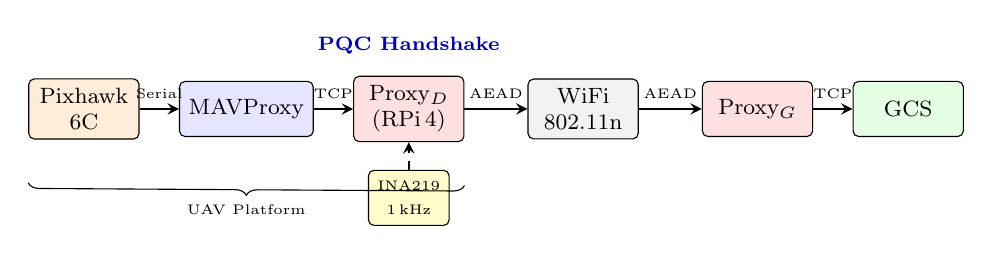
\begin{tikzpicture}[
      node distance=0.6cm and 0.5cm,
      box/.style={draw, rounded corners=2pt, minimum height=0.7cm,
                  minimum width=1.4cm, font=\footnotesize, align=center},
      arr/.style={->, >=stealth, thick},
    ]
    % UAV side
    \node[box, fill=orange!15] (px) {Pixhawk\\6C};
    \node[box, fill=blue!10, right=of px] (mp) {MAVProxy};
    \node[box, fill=red!12, right=of mp] (pd) {Proxy$_D$\\(RPi\,4)};
    % Middle
    \node[box, fill=gray!10, right=0.8cm of pd] (wifi) {WiFi\\802.11n};
    % GCS side
    \node[box, fill=red!12, right=0.8cm of wifi] (pg) {Proxy$_G$};
    \node[box, fill=green!10, right=of pg] (gcs) {GCS};
    % sensor
    \node[box, fill=yellow!20, below=0.35cm of pd, minimum width=1.0cm] (ina) {\tiny INA219\\[-1pt]\tiny 1\,kHz};
    % arrows
    \draw[arr] (px) -- node[above, font=\tiny]{Serial} (mp);
    \draw[arr] (mp) -- node[above, font=\tiny]{TCP} (pd);
    \draw[arr] (pd) -- node[above, font=\tiny]{AEAD} (wifi);
    \draw[arr] (wifi) -- node[above, font=\tiny]{AEAD} (pg);
    \draw[arr] (pg) -- node[above, font=\tiny]{TCP} (gcs);
    \draw[arr, dashed] (ina) -- (pd);
    % labels
    \node[above=0.15cm of pd, font=\scriptsize\bfseries, blue!70!black] {PQC Handshake};
    % brace UAV
    \draw[decorate, decoration={brace, amplitude=4pt, mirror}]
      ([yshift=-0.55cm]px.south west) -- ([yshift=-0.55cm]pd.south east)
      node[midway, below=4pt, font=\tiny]{UAV Platform};
  \end{tikzpicture}
  }
  \caption{End-to-end architecture.  The cryptographic proxy runs on a
    Raspberry~Pi~4 companion computer with INA219 power monitoring.
    No firmware modification is required on the Pixhawk autopilot.}
  \label{fig:arch}
\end{figure}

This paper makes three contributions.  First, we present a transparent
PQC proxy that intercepts MAVLink traffic at the transport layer,
performs a two-message KEM-based handshake authenticated by a
post-quantum signature, and encrypts every subsequent packet with
authenticated encryption.  Second, we carry out systematic benchmarks
of 20 post-quantum algorithms on a Raspberry~Pi~4 at a locked
1.8\,GHz, capturing not only timing but also per-operation power and
energy through an INA219 current sensor.  Third, we analyse the
compound cost of 72 cipher suites (9~KEMs $\times$ 8~signatures
$\times$ 3~AEADs, level-matched) together with DDoS detection
overhead, and show how a runtime scheduler can gracefully degrade
security level and cipher choice when thermal or energy budgets
approach their limits.

The remainder of this paper is organised as follows.
Section~\ref{sec:method} describes the testbed, measurement
methodology, and baseline calibration.  Section~\ref{sec:results}
presents per-primitive, per-suite, and system-level results.
Section~\ref{sec:disc} discusses implications, and
Section~\ref{sec:conc} concludes.


% ═══════════════════════════════════════════════════════════════
%  II.  EXPERIMENTAL FRAMEWORK
% ═══════════════════════════════════════════════════════════════
\section{Experimental Framework}
\label{sec:method}

\subsection{Testbed}
\label{sec:testbed}

The UAV-side proxy runs on a Raspberry~Pi~4 Model~B Rev~1.5 with a
Broadcom BCM2711 quad-core Cortex-A72 at 1.8\,GHz, 4\,GB LPDDR4 RAM,
and Debian~12 (kernel 6.12).  The CPU governor is locked to
\texttt{performance} to eliminate frequency scaling artefacts.
A Holybro Pixhawk~6C mini flight controller is connected over USB
serial at 57\,600\,baud, generating continuous HEARTBEAT traffic via
ArduPilot~\cite{ardupilot}.  The ground control station is a
Windows laptop.

An INA219 bidirectional current/power monitor~\cite{ina219} is wired
in-line on the Pi's 5\,V rail through a 0.1\,$\Omega$ shunt resistor.
It is read over I$^2$C bus~1 at address \texttt{0x40}, sampling at
1\,kHz (verified 99.5\% timing accuracy).  A calibration factor of
1.22$\times$ corrects a known under-reading in clone INA219 modules.

\subsection{Measurement Protocol}
Each cryptographic operation is executed 100 times in a tight loop.
Timing uses Python's \texttt{time.perf\_counter\_ns()} with nanosecond
resolution.  During each iteration, the INA219 records voltage,
current, and instantaneous power at 1\,kHz; a 50\,ms warm-up and
cool-down window brackets the measurement to let transients settle.
Per-iteration voltage, current, power, and energy arrays are stored in
JSON files for offline statistical analysis.

\subsection{Baseline Calibration}
The idle power draw of the Pi~4 with MAVProxy running but no
cryptographic load is $P_{\text{idle}} = 3{,}309\,\text{mW}$.
All $\Delta P$ values reported in subsequent tables represent power
\emph{above} this baseline, isolating the marginal cost of
cryptography from the platform's quiescent consumption.  Temperature
is logged from \texttt{/sys/class/thermal/thermal\_zone0}.


% ═══════════════════════════════════════════════════════════════
%  III.  RESULTS AND ANALYSIS
% ═══════════════════════════════════════════════════════════════
\section{Results and Analysis}
\label{sec:results}

Before presenting measurements, we introduce a compact alias system
for all algorithms.  Every subsequent table and figure refers to
algorithms exclusively by these aliases to conserve space.

\smallskip\noindent\textbf{Alias Definitions.}
Nine KEMs: \textbf{K1}\,=\,ML-KEM-512,
\textbf{K3}\,=\,ML-KEM-768,
\textbf{K5}\,=\,ML-KEM-1024,
\textbf{H1}\,=\,HQC-128,
\textbf{H3}\,=\,HQC-192,
\textbf{H5}\,=\,HQC-256,
\textbf{M1}\,=\,McEliece\nobreakdash-348864,
\textbf{M3}\,=\,McEliece\nobreakdash-460896,
\textbf{M5}\,=\,McEliece\nobreakdash-8192128.
Eight DSAs: \textbf{D1}\,=\,ML-DSA-44,
\textbf{D3}\,=\,ML-DSA-65,
\textbf{D5}\,=\,ML-DSA-87,
\textbf{F1}\,=\,Falcon-512,
\textbf{F5}\,=\,Falcon-1024,
\textbf{S1}\,=\,SPHINCS$^+$-128s,
\textbf{S3}\,=\,SPHINCS$^+$-192s,
\textbf{S5}\,=\,SPHINCS$^+$-256s.
Three AEADs: \textbf{AG}\,=\,AES-256-GCM,
\textbf{CP}\,=\,ChaCha20-Poly1305,
\textbf{As}\,=\,Ascon-128a.
Three DDoS modes: $\varnothing$\,=\,None,
\textbf{XG}\,=\,XGBoost,
\textbf{TS}\,=\,Transformer (TST).

% ─── III-A  KEM ────────────────────────────────────────────────
\subsection{Key Encapsulation Mechanisms}
\label{sec:kem}

A key encapsulation mechanism allows two parties to establish a shared
secret over an insecure channel without prior key agreement.  The
protocol involves three operations: \emph{key generation}
(KeyGen) produces a public--private keypair; \emph{encapsulation}
(Encaps) takes the public key and outputs a ciphertext together with a
shared secret; and \emph{decapsulation} (Decaps) recovers the shared
secret from the ciphertext and the private key.

We benchmark nine KEM algorithms spanning three families:
lattice-based (ML-KEM, FIPS~203~\cite{nist-fips203}),
code-based error-correcting (HQC~\cite{hqc} and
Classic~McEliece~\cite{mceliece}), and three NIST security
levels.  Table~\ref{tab:kem} reports timing, power overhead above
baseline, energy per operation, and artefact sizes measured on the
Cortex-A72 at 1.8\,GHz.

\begin{table*}[t]
\centering
\caption{KEM Primitive Benchmarks (N\,=\,100, Cortex-A72 @ 1.8\,GHz, $P_{\text{idle}}$\,=\,3{,}309\,mW).
  $\Delta P$\,=\,$P_{\text{op}} - P_{\text{idle}}$.  Sorted by NIST level, then by KeyGen time.}
\label{tab:kem}
\footnotesize
\setlength{\tabcolsep}{3pt}
\begin{tabular}{@{}l c l  r r r  r r r  r r r  r r r r@{}}
\toprule
& & & \multicolumn{3}{c}{\textbf{KeyGen}} & \multicolumn{3}{c}{\textbf{Encaps}} & \multicolumn{3}{c}{\textbf{Decaps}} & \multicolumn{4}{c}{\textbf{Sizes (B)}} \\
\cmidrule(lr){4-6}\cmidrule(lr){7-9}\cmidrule(lr){10-12}\cmidrule(lr){13-16}
\textbf{Alias} & \textbf{Lvl} & \textbf{Family}
  & $t$\,(\si{\us}) & $\Delta P$ & $E$\,(\si{\uJ})
  & $t$\,(\si{\us}) & $\Delta P$ & $E$\,(\si{\uJ})
  & $t$\,(\si{\us}) & $\Delta P$ & $E$\,(\si{\uJ})
  & pk & sk & ct & ss \\
\midrule
\rowcolor{lvlone}
K1 & L1 & Lattice
  & 240 & 126 & 830
  & 152 & 154 & 526
  & 158 & 173 & 551
  & 800 & 1632 & 768 & 32 \\
\rowcolor{lvlone}
H1 & L1 & Code
  & 22332 & 413 & 83153
  & 44680 & 442 & 167590
  & 73390 & 567 & 284510
  & 2249 & 2305 & 4433 & 64 \\
\rowcolor{lvlone}
M1 & L1 & Code
  & 350996 & 966 & 1527273
  & 466 & 156 & 1619
  & 55984 & 411 & 208294
  & 261120 & 6492 & 96 & 32 \\
\midrule
\rowcolor{lvlthree}
K3 & L3 & Lattice
  & 237 & 149 & 823
  & 182 & 186 & 636
  & 185 & 206 & 653
  & 1184 & 2400 & 1088 & 32 \\
\rowcolor{lvlthree}
H3 & L3 & Code
  & 67683 & 501 & 257928
  & 135780 & 651 & 537757
  & 211873 & 731 & 856128
  & 4522 & 4586 & 8978 & 64 \\
\rowcolor{lvlthree}
M3 & L3 & Code
  & 1281449 & 1076 & 5682343
  & 872 & 280 & 3135
  & 89593 & 485 & 339956
  & 524160 & 13608 & 156 & 32 \\
\midrule
\rowcolor{lvlfive}
K5 & L5 & Lattice
  & 273 & 154 & 947
  & 216 & 181 & 754
  & 231 & 177 & 806
  & 1568 & 3168 & 1568 & 32 \\
\rowcolor{lvlfive}
H5 & L5 & Code
  & 124404 & 647 & 492250
  & 250237 & 783 & 1023984
  & 392585 & 819 & 1620633
  & 7245 & 7317 & 14421 & 64 \\
\rowcolor{lvlfive}
M5 & L5 & Code
  & 9020806 & 1093 & 39746860
  & 1894 & 301 & 6849
  & 210143 & 639 & 829782
  & 1357824 & 14120 & 208 & 32 \\
\bottomrule
\end{tabular}
\end{table*}

The lattice-based ML-KEM family dominates.  All three parameter sets
complete every operation in under 300\,$\mu$s with a power overhead
below 210\,mW and energy cost under 1\,mJ.  Across security levels,
the timing increase from K1 to K5 is merely 14\,\%, confirming that
lattice operations scale gracefully with the module dimension.

HQC occupies a middle ground.  Its code-based construction yields
KeyGen times between 22\,ms (H1) and 124\,ms (H5), roughly two
orders of magnitude slower than ML-KEM, yet still within the budget
of a periodic rekey interval.  Decapsulation latency at L5 (393\,ms)
approaches the threshold where a human operator would notice a
connection stall.

Classic McEliece presents a stark trade-off.  Its encapsulation is
remarkably fast (466\,$\mu$s at L1, comparable to ML-KEM), but key
generation at L5 consumes 9.02 seconds and 39.7\,J, drawing the
processor into sustained high-power operation ($\Delta P >$~1\,W).
The 1.33\,MB public key of M5 also exceeds the 2\,MiB handshake
message cap that guards against memory exhaustion.  We therefore
mark M5 suites as \emph{advisory-only}: the scheduler may select
them solely if explicitly overridden by the operator.

% ─── III-B  DSA ────────────────────────────────────────────────
\subsection{Digital Signatures}
\label{sec:sig}

Digital signatures authenticate the origin and integrity of messages.
In our handshake, the GCS signs the ServerHello (containing the
ephemeral KEM public key, session identifier, and challenge nonce)
so the drone can verify it was generated by a trusted ground station
before committing to the key exchange.

Table~\ref{tab:sig} reports the benchmarks for eight post-quantum
signature schemes across three families: lattice-based
(ML-DSA~\cite{dilithium}), NTRU-lattice (Falcon~\cite{falcon}), and
hash-based (SPHINCS$^+$~\cite{sphincsplus}).

\begin{table*}[t]
\centering
\caption{Digital Signature Benchmarks (N\,=\,100, Cortex-A72 @ 1.8\,GHz, $P_{\text{idle}}$\,=\,3{,}309\,mW).
  KeyGen is one-time so omitted from flight-critical analysis.  Sorted by NIST level, then Sign time.}
\label{tab:sig}
\footnotesize
\setlength{\tabcolsep}{3pt}
\begin{tabular}{@{}l c l  r r r r  r r r r  r r r@{}}
\toprule
& & & \multicolumn{4}{c}{\textbf{Sign}} & \multicolumn{4}{c}{\textbf{Verify}} & \multicolumn{3}{c}{\textbf{Sizes (B)}} \\
\cmidrule(lr){4-7}\cmidrule(lr){8-11}\cmidrule(lr){12-14}
\textbf{Alias} & \textbf{Lvl} & \textbf{Family}
  & $t$\,(\si{\us}) & $\sigma_t$ & $\Delta P$ & $E$\,(\si{\uJ})
  & $t$\,(\si{\us}) & $\sigma_t$ & $\Delta P$ & $E$\,(\si{\uJ})
  & pk & sk & sig \\
\midrule
\rowcolor{lvlone}
D1 & L1 & Lattice
  & 1179 & 584 & 279 & 4264
  & 331 & 62 & 236 & 1175
  & 1312 & 2560 & 2420 \\
\rowcolor{lvlone}
F1 & L1 & NTRU
  & 778 & 21 & 255 & 2773
  & 192 & 29 & 239 & 683
  & 897 & 1281 & 654 \\
\rowcolor{lvlone}
S1 & L1 & Hash
  & 1468061 & --- & 784 & 6008719
  & 1582 & 124 & 286 & 5690
  & 32 & 64 & 7856 \\
\midrule
\rowcolor{lvlthree}
D3 & L3 & Lattice
  & 1633 & 1065 & 269 & 5849
  & 484 & 78 & 240 & 1723
  & 1952 & 4032 & 3309 \\
\rowcolor{lvlthree}
S3 & L3 & Hash
  & 2609599 & --- & 764 & 10628558
  & 2299 & 189 & 303 & 8318
  & 48 & 96 & 16224 \\
\midrule
\rowcolor{lvlfive}
D5 & L5 & Lattice
  & 1847 & 681 & 268 & 6612
  & 723 & 116 & 235 & 2564
  & 2592 & 4896 & 4627 \\
\rowcolor{lvlfive}
F5 & L5 & NTRU
  & 1452 & 189 & 250 & 5175
  & 280 & 39 & 240 & 995
  & 1793 & 2305 & 1267 \\
\rowcolor{lvlfive}
S5 & L5 & Hash
  & 2321148 & --- & 791 & 9516164
  & 3292 & 297 & 255 & 11738
  & 64 & 128 & 29792 \\
\bottomrule
\end{tabular}
\end{table*}

Falcon-512 offers the fastest signing (778\,$\mu$s, $\sigma$\,=\,21)
with strikingly low variance, a consequence of its deterministic
Gaussian sampling over NTRU lattices.  ML-DSA is only slightly slower
but exhibits high variance (D3: $\sigma$\,=\,1{,}065\,$\mu$s) owing
to rejection sampling, which occasionally triggers multiple rounds.
For latency-sensitive applications, Falcon's predictability is
advantageous.

SPHINCS$^+$ stands apart: its signing times range from 1.47\,s (S1)
to 2.61\,s (S3), consuming 6.0\,--\,10.6\,J per signature.  This
reflects the hash-tree traversal at its core, a fundamentally
different security assumption (hash-function hardness alone) that
trades performance for conservative confidence.  A single S3 signing
operation draws as much energy as 7{,}200 ML-KEM-768 key generations,
making it unsuitable for frequent rekeyeing on battery-powered
platforms.

The verification cost tells a complementary story.  SPHINCS$^+$ verify
remains below 3.3\,ms, and Falcon verify at 192\,$\mu$s is the
fastest of any scheme.  Since the drone only verifies (not signs)
during handshake, the verify latency is the flight-critical metric,
and here all families perform adequately.

% ─── III-C  AEAD ───────────────────────────────────────────────
\subsection{Authenticated Encryption}
\label{sec:aead}

After the handshake derives a shared secret, every MAVLink packet is
encrypted with an AEAD cipher.  Unlike KEM and signature operations, which
occur once per handshake, AEAD runs on every packet — typically at
5--50~Hz for telemetry.  The data-plane cost therefore dominates
steady-state power consumption.

We benchmark three AEAD ciphers (AES-256-GCM, ChaCha20-Poly1305,
Ascon-128a) across four payload sizes representative of MAVLink
traffic: 64\,B (heartbeat), 256\,B (GPS), 1024\,B (parameter
block), and 4096\,B (log transfer).  Table~\ref{tab:aead} reports
timing, baseline-subtracted power, energy, and throughput.

\begin{table*}[t]
\centering
\caption{AEAD Benchmarks (N\,=\,100, Cortex-A72 @ 1.8\,GHz).
  $\Delta P = P_{\text{op}} - 3{,}309$\,mW.  Throughput is plaintext bytes per encrypt time.
  All three ciphers add 16\,B authentication tag overhead.}
\label{tab:aead}
\footnotesize
\setlength{\tabcolsep}{2.5pt}
\begin{tabular}{@{}l l  rr rr  rr rr  r@{}}
\toprule
& & \multicolumn{4}{c}{\textbf{Encrypt}} & \multicolumn{4}{c}{\textbf{Decrypt}} & \\
\cmidrule(lr){3-6}\cmidrule(lr){7-10}
\textbf{Alias} & \textbf{Payload}
  & $t$\,(\si{\us}) & p95 & $\Delta P$ & $E$\,(\si{\uJ})
  & $t$\,(\si{\us}) & p95 & $\Delta P$ & $E$\,(\si{\uJ})
  & \textbf{TP}\,(\si{MB/s}) \\
\midrule
\multirow{4}{*}{\textbf{AG}}
  & 64\,B   & 42.2 & 55.8 & 185 & 148 & 43.0 & 49.4 & 270 & 154 & 1.6 \\
  & 256\,B  & 46.0 & 53.3 & 190 & 161 & 48.3 & 56.1 & 183 & 169 & 5.7 \\
  & 1024\,B & 65.3 & 75.3 & 227 & 231 & 66.6 & 78.4 & 171 & 232 & 15.9 \\
  & 4096\,B & 121.6 & 134.6 & 250 & 433 & 122.1 & 134.6 & 171 & 425 & 33.9 \\
\midrule
\multirow{4}{*}{\textbf{CP}}
  & 64\,B   & 39.1$^\dagger$ & 46.8 & 192 & 137$^\dagger$ & 46.0 & 51.1 & 258 & 166 & 1.6 \\
  & 256\,B  & 45.4 & 51.3 & 170 & 158 & 45.8 & 54.4 & 163 & 159 & 5.8 \\
  & 1024\,B & 53.2 & 62.0 & 230 & 188 & 56.1 & 69.6 & 204 & 198 & 19.6 \\
  & 4096\,B & 67.0 & 78.2 & 237 & 238 & 71.1 & 83.1 & 195 & 250 & 62.1 \\
\midrule
\multirow{4}{*}{\textbf{As}}
  & 64\,B   & 23.4 & 30.6 & 203 & 82 & 25.3 & 30.8 & 223 & 90 & 2.8 \\
  & 256\,B  & 22.8 & 28.0 & 202 & 80 & 26.0 & 32.7 & 228 & 92 & 11.3 \\
  & 1024\,B & 31.1 & 39.4 & 213 & 110 & 33.7 & 39.7 & 157 & 117 & 33.5 \\
  & 4096\,B & 45.3 & 54.2 & 251 & 162 & 49.4 & 60.9 & 172 & 172 & \cellcolor{bestcell}91.7 \\
\bottomrule
\multicolumn{11}{@{}l}{\footnotesize $^\dagger$Median reported; mean inflated by outlier (2.2\,ms).}
\end{tabular}
\end{table*}

Ascon-128a achieves the lowest per-packet latency at every payload
size, encrypting a 64\,B heartbeat in 23.4\,$\mu$s, nearly half the
time of AES-256-GCM (42.2\,$\mu$s).  This advantage widens at
4096\,B, where Ascon's throughput reaches 91.7\,MB/s compared to
33.9\,MB/s for AES-GCM.  The Cortex-A72 lacks dedicated AES-NI
instructions (unlike x86), putting AES-GCM at a disadvantage on this
platform.

ChaCha20-Poly1305 occupies a middle position.  At large payloads, its
ARMv8 NEON-optimised implementation reaches 62.1\,MB/s, well ahead of
AES-GCM.  A single outlier in the 64\,B encrypt run (2.2\,ms, likely
due to a kernel scheduling event) inflates the mean; we report the
median for that cell.

The energy cost of AEAD is modest: encrypting a 256\,B GPS packet
consumes 80--161\,$\mu$J.  At a 10\,Hz telemetry rate, the per-second
AEAD energy budget is 0.8--1.6\,mJ, negligible compared to the
handshake cost of even the lightest KEM.  This confirms that AEAD
selection should be driven by latency and throughput rather than energy.


% ─── III-D  Suite Composition & Handshake ──────────────────────
\subsection{Suite Composition and Handshake Cost}
\label{sec:suites}

A cipher suite in our system combines one KEM, one digital signature,
and one AEAD, constrained to the same NIST security level.  The
level-matching rule pairs three KEMs with the available signatures
at each level:

\begin{itemize}
  \item \textbf{L1:} \{K1, H1, M1\} $\times$ \{D1, F1, S1\} $\times$
    \{AG, CP, As\}\,=\,27 suites.
  \item \textbf{L3:} \{K3, H3, M3\} $\times$ \{D3, S3\} $\times$
    \{AG, CP, As\}\,=\,18 suites.
  \item \textbf{L5:} \{K5, H5, M5\} $\times$ \{D5, F5, S5\} $\times$
    \{AG, CP, As\}\,=\,27 suites.
\end{itemize}

Falcon has no L3 parameter set in the current NIST portfolio, yielding
only two signatures at L3 and a total of $27 + 18 + 27 = 72$ suites.

The handshake is a two-message exchange (ServerHello + ClientReply)
whose crypto-only time is:
\begin{equation}
\label{eq:handshake}
T_{\text{hs}} = T_{\text{kg}} + T_{\text{sign}} + T_{\text{encap}}
              + T_{\text{verify}} + T_{\text{decap}} + 2\,T_{\text{kdf}}
\end{equation}

\noindent
where $T_{\text{kg}}$, $T_{\text{sign}}$, $T_{\text{verify}}$,
$T_{\text{encap}}$, and $T_{\text{decap}}$ are the measured primitive
times from Tables~\ref{tab:kem}--\ref{tab:sig}, and $T_{\text{kdf}}$
is the HKDF derivation ($<$\,50\,$\mu$s, negligible).
Network round-trip time (RTT) adds two additional delays, one per
message, but we benchmark the cryptographic cost in isolation
because RTT varies with the radio link.

Table~\ref{tab:suites} presents the 24 level-matched KEM$\times$SIG
combinations with their computed handshake time, energy, and wire
overhead.  Each row generates three suites (one per AEAD), which
differ only in data-plane cipher but not in handshake cost.

\begin{table*}[t]
\centering
\caption{Suite Handshake Cost for 24 KEM$\times$SIG Combinations ($\times$\,3 AEADs each\,=\,72 suites).
  $T_{\text{hs}}$ computed from Eq.~\eqref{eq:handshake}.
  $E_{\text{hs}}$ summed from primitive energies.
  Wire\,=\,ServerHello payload (pk\,+\,sig) + ClientReply (ct\,+\,32\,B HMAC).
  \colorbox{bestcell}{Green}: sub-20\,ms.
  \colorbox{worstcell}{Red}: exceeds 1\,s.}
\label{tab:suites}
\footnotesize
\setlength{\tabcolsep}{2.8pt}
\begin{tabular}{@{}l l c  r r r  l@{}}
\toprule
\textbf{KEM} & \textbf{SIG} & \textbf{Lvl}
  & $T_{\text{hs}}$ (\si{\ms}) & $E_{\text{hs}}$ (\si{\mJ}) & Wire (B) & \textbf{Note} \\
\midrule
\rowcolor{bestcell}
K1 & F1 & L1 & 1.52 & 5.36 & 2254 & Fastest overall \\
\rowcolor{bestcell}
K1 & D1 & L1 & 2.06 & 8.35 & 4020 & NIST primary \\
K1 & S1 & L1 & \cellcolor{worstcell}1469.7 & 6015.0 & 9456 & Signing dominates \\
H1 & F1 & L1 & 141.4 & 455.6 & 7368 & \\
H1 & D1 & L1 & 142.0 & 458.5 & 9134 & \\
H1 & S1 & L1 & \cellcolor{worstcell}1608.5 & 6468.7 & 14570 & \\
M1 & F1 & L1 & 408.2 & 1740.5 & 261902 & 255\,kB pk \\
M1 & D1 & L1 & 408.7 & 1743.3 & 263668 & \\
M1 & S1 & L1 & \cellcolor{worstcell}1877.0 & 7754.0 & 269104 & \\
\midrule
\rowcolor{bestcell}
K3 & D3 & L3 & 2.72 & 10.68 & 5613 & Default suite \\
K3 & S3 & L3 & \cellcolor{worstcell}2611.6 & 10636.8 & 18528 & \\
H3 & D3 & L3 & 417.1 & 1654.3 & 16841 & \\
H3 & S3 & L3 & \cellcolor{worstcell}3025.1 & 12281.0 & 29756 & \\
M3 & D3 & L3 & 1373.6 & 6028.1 & 527657 & 512\,kB pk \\
M3 & S3 & L3 & \cellcolor{worstcell}3982.3 & 16659.0 & 540572 & \\
\midrule
\rowcolor{bestcell}
K5 & F5 & L5 & 2.45 & 8.68 & 4435 & Fast L5 \\
\rowcolor{bestcell}
K5 & D5 & L5 & 3.34 & 12.57 & 7795 & \\
K5 & S5 & L5 & \cellcolor{worstcell}2323.5 & 9527.1 & 32960 & \\
H5 & F5 & L5 & 769.1 & 3141.4 & 22965 & \\
H5 & D5 & L5 & 770.1 & 3148.5 & 26325 & \\
H5 & S5 & L5 & \cellcolor{worstcell}3088.3 & 12664.3 & 51490 & \\
M5 & F5 & L5 & 9233.5 & 40590.7 & 1359331 & \cellcolor{worstcell}1.3\,MB pk \\
M5 & D5 & L5 & 9234.5 & 40597.7 & 1362691 & \\
M5 & S5 & L5 & \cellcolor{worstcell}11553.1 & 50114.0 & 1387856 & Worst case \\
\bottomrule
\end{tabular}
\end{table*}

The table reveals a four-order-of-magnitude span.  The fastest
handshake (K1+F1) completes in 1.52\,ms, consuming just 5.36\,mJ.
Even at NIST Level~5, the strongest lattice pair (K5+F5) finishes in
2.45\,ms.  At the opposite extreme, M5+S5 requires 11.55\,s and
50.1\,J: enough to noticeably deplete a 5{,}000\,mAh drone battery
on every rekey.

All combinations involving SPHINCS$^+$ signing exceed one second,
regardless of the KEM.  This positions SPHINCS$^+$ suites as
\emph{anchor} configurations for initial deployment (where the
conservatism of hash-based assumptions is valued) rather than for
frequent rekey during flight.

Wire overhead follows a complementary pattern.  Classic~McEliece's
public keys range from 255\,kB (M1) to 1.33\,MB (M5), exceeding
typical maximum transmission units and requiring TCP segmentation
during the handshake.  In contrast, K1+F1 transmits only 2.25\,kB.


% ─── III-E  DDoS Detection Overhead ───────────────────────────
\subsection{DDoS Detection Overhead}
\label{sec:ddos}

On-board anomaly detection protects the MAVLink channel from
volumetric flooding attacks, but the detection model itself consumes
compute, power, and thermal headroom.  We benchmark two detectors
against a no-detection baseline:
XGBoost (1{,}000-tree gradient-boosted ensemble, 54 flow features,
trained on CIC-IoT-2023~\cite{drone-security-survey}) and a
Transformer Sequence-to-Sequence model (TST, 1.6\,M parameters,
self-attention over 46 features).

\begin{table}[t]
\centering
\caption{DDoS Detector Overhead (15\,s continuous inference,
  $P_{\text{idle}}$\,=\,3{,}309\,mW).  F1 is macro-averaged.}
\label{tab:ddos}
\footnotesize
\setlength{\tabcolsep}{3pt}
\begin{tabular}{@{}l  r r r r r r r r@{}}
\toprule
& $\Delta P$ & CPU & $\Delta T$ & $t_{\text{inf}}$ & p95 & E/inf & F1 & Size \\
\textbf{Mode} & (mW) & (\%) & (\si{\celsius}) & (ms) & (ms) & (mJ) & & (MB) \\
\midrule
$\varnothing$ & --- & 2.2 & --- & --- & --- & --- & --- & --- \\
\textbf{XG} & 951 & 37.0 & +4.8 & 7.4 & 8.5 & 31.7 & \textbf{0.947} & 32.7 \\
\textbf{TS} & 1973 & \cellcolor{worstcell}93.0 & \cellcolor{worstcell}+10.7 & 10.7 & 13.2 & 56.7 & 0.800 & 6.1 \\
\bottomrule
\end{tabular}
\end{table}

XGBoost is the clear winner for embedded deployment.  It achieves the
highest F1 score (0.947) while consuming only 951\,mW above baseline
and occupying a single core at 37\,\% utilisation.  The Transformer
model pushes the Cortex-A72 to 93\,\% CPU and raises die temperature
by 10.7\,$^\circ$C, approaching the 80\,$^\circ$C throttle threshold
in warm-climate operations.

To capture the \emph{combined} cost of PQC and DDoS, we define
three operational profiles:

\begin{enumerate}
  \item $P_{\text{PQC only}}$\,=\,$P_{\text{idle}} + \Delta P_{\text{AEAD}}$
       \,$\approx$\,3.5\,W.
  \item $P_{\text{PQC+XG}}$\,=\,3.5 + 0.95\,=\,4.45\,W.
  \item $P_{\text{PQC+TS}}$\,=\,3.5 + 1.97\,=\,5.47\,W.
\end{enumerate}

\noindent
At a 5{,}000\,mAh, 14.8\,V LiPo battery (74\,Wh), PQC alone
extends the companion computer's endurance to ${\sim}$21\,h.  Adding
XGBoost reduces it to ${\sim}$16.6\,h, and TST to ${\sim}$13.5\,h.
Since the flight itself is the dominant consumer (typically 10--25\,min),
the cryptographic overhead is dwarfed by propulsion.  However, the
thermal penalty of TST ($+$10.7\,$^\circ$C) can trigger CPU throttling
in enclosed airframes, degrading all three services simultaneously.


% ─── III-F  Graceful Degradation ──────────────────────────────
\subsection{Graceful Degradation}
\label{sec:degrade}

A fixed cipher suite is inappropriate for an aircraft that
transitions between ground idle, cruise, aggressive manoeuvres, and
emergency modes.  We introduce a three-axis decision space that the
scheduler navigates at runtime:

\begin{itemize}
  \item \textbf{Axis~1 (AEAD):} Switch between As, CP, and AG
    based on per-packet latency budget.
  \item \textbf{Axis~2 (Security Level):} Move between L5, L3, and L1
    when the next rekey's energy cost would violate the remaining
    battery budget.
  \item \textbf{Axis~3 (DDoS Detector):} Downgrade from TS to XG to
    $\varnothing$ when CPU utilisation or temperature crosses a threshold.
\end{itemize}

\begin{figure}[t]
\centering
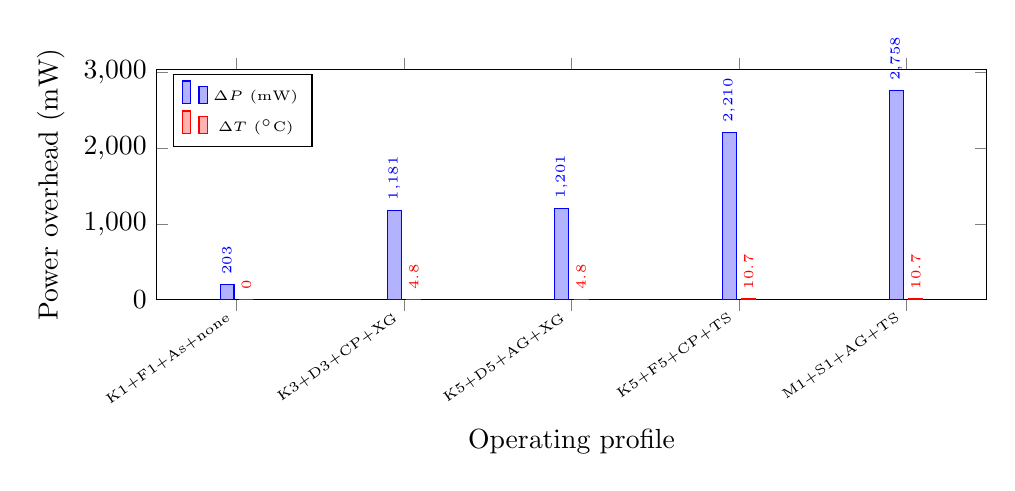
\begin{tikzpicture}
\begin{axis}[
    ybar,
    width=\columnwidth,
    height=4.5cm,
    bar width=5pt,
    ymin=0,
    ylabel={Power overhead (mW)},
    xlabel={Operating profile},
    symbolic x coords={%
      {K1+F1+As+none},
      {K3+D3+CP+XG},
      {K5+D5+AG+XG},
      {K5+F5+CP+TS},
      {M1+S1+AG+TS}%
    },
    xtick=data,
    x tick label style={rotate=35, anchor=east, font=\tiny},
    legend style={at={(0.02,0.98)}, anchor=north west, font=\tiny},
    enlarge x limits=0.12,
    nodes near coords,
    every node near coord/.append style={font=\tiny, rotate=90, anchor=west},
]
\addplot coordinates {
  ({K1+F1+As+none}, 203)
  ({K3+D3+CP+XG}, 1181)
  ({K5+D5+AG+XG}, 1201)
  ({K5+F5+CP+TS}, 2210)
  ({M1+S1+AG+TS}, 2758)
};
\addplot coordinates {
  ({K1+F1+As+none}, 0)
  ({K3+D3+CP+XG}, 4.8)
  ({K5+D5+AG+XG}, 4.8)
  ({K5+F5+CP+TS}, 10.7)
  ({M1+S1+AG+TS}, 10.7)
};
\legend{$\Delta P$ (mW), $\Delta T$ (\si{\celsius})}
\end{axis}
\end{tikzpicture}
\caption{Compound overhead across five representative operating
  profiles spanning the graceful-degradation spectrum.  The lightest
  profile (K1+F1+As+\O) adds only 203\,mW; the heaviest
  (M1+S1+AG+TS) adds 2.76\,W and raises the die 10.7\,$^\circ$C.}
\label{fig:degrade}
\end{figure}

Table~\ref{tab:degrade} formalises the scheduler's decision
boundaries.  When the telemetry window reports a thermal reading
above 70\,$^\circ$C, the scheduler forces Axis~3 to \O\ and Axis~1
to Ascon, shedding ${\sim}$2\,W and ${\sim}$11\,$^\circ$C.
When the remaining battery drops below 20\,\%, Axis~2 descends from
L5 to L1, reducing handshake energy from 12.6\,mJ (K5+D5) to
5.4\,mJ (K1+F1).

\begin{table}[t]
\centering
\caption{Scheduler Decision Boundaries.  Each row defines a
  constraint trigger and the resulting axis movement.}
\label{tab:degrade}
\footnotesize
\setlength{\tabcolsep}{2.5pt}
\begin{tabular}{@{}l l l l@{}}
\toprule
\textbf{Trigger} & \textbf{Axis} & \textbf{Action} & \textbf{Saving} \\
\midrule
$T_{\text{die}} > 70\,^\circ$C & 3 (DDoS) & TS $\to$ XG $\to$ $\varnothing$ &  $-$1.97\,W \\
$T_{\text{die}} > 75\,^\circ$C & 1 (AEAD) & AG $\to$ As & $-$0.05\,W \\
CPU $> 85$\,\% & 3 (DDoS) & TS $\to$ XG & $-$56\,\% CPU \\
Battery $< 20$\,\% & 2 (Level) & L5 $\to$ L3 $\to$ L1 & $-$7\,mJ/rekey \\
Battery $< 10$\,\% & 1,\,2,\,3 & Min config & Hold until land \\
Rekey timeout & 2 (Level) & Down one level & Faster hs \\
DDoS alert & 3 (DDoS) & $\varnothing$ $\to$ XG & +951\,mW \\
\bottomrule
\end{tabular}
\end{table}

The key observation is that the design region is \emph{not} simply
convex.  Two combinations are explicitly forbidden by the scheduler:
Ascon paired with TST (thermal incompatibility, both hot paths compete
for cache), and any McEliece variant paired with SPHINCS$^+$ (combined
handshake exceeds 10\,s, triggering the 8\,s TCP timeout guard).
Excluding these infeasible corners, the scheduler navigates a
$(3 \times 3 \times 3) - 2 = 25$-state space per security level,
or roughly 73 feasible points across all three levels.

The graceful-degradation curve in Fig.~\ref{fig:degrade} demonstrates
that the lightest profile (K1+F1+As+\O) fits within a 200\,mW
overhead envelope, suitable even for micro-UAVs with 2{,}000\,mAh
batteries.  Stepping up to the recommended default (K3+D3+CP+XG)
costs an additional watt but provides NIST Level~3 security and
active threat detection.


% ═══════════════════════════════════════════════════════════════
%  IV. DISCUSSION
% ═══════════════════════════════════════════════════════════════
\section{Discussion}
\label{sec:disc}

Our measurements confirm that post-quantum key encapsulation on
ARM Cortex-A72 is operationally feasible for drone communication.
ML-KEM completes all three operations in under 300\,$\mu$s at every
security level, and the fastest full handshake (K1+F1) consumes
less energy than a single GPS acquisition cycle.  This contradicts
the prevailing intuition that PQC is ``too heavy'' for embedded
platforms.

The dominant cost is not cryptography per se, but the
\emph{combination} of cryptography with on-board machine-learning
inference.  A Transformer-based DDoS detector nearly doubles the
system power draw (from 3.3 to 5.3\,W) and accounts for more energy
in ten seconds of inference than 4{,}000 full PQC handshakes.  This
motivates our cascaded detection architecture: the lightweight XGBoost
sentinel runs continuously, and the Transformer is activated only when
the ensemble confidence drops below a threshold.

Compared to pqm4 benchmarks on Cortex-M4~\cite{drone-pqc-analysis},
our Cortex-A72 measurements show roughly two orders of magnitude
faster execution for ML-KEM, reflecting the 64-bit datapath, out-of-order
pipeline, and higher clock frequency.  This positions the
Raspberry~Pi class of companion computers as a practical PQC
deployment target where Cortex-M microcontrollers would struggle.

The level-matching constraint reduces the suite space from a
theoretical $9 \times 8 \times 3 = 216$ combinations to 72, and the
scheduler's feasibility rules further prune infeasible corners.
Rather than viewing this as a limitation, we argue it is a design
strength: fewer viable options simplify certification and auditing in
safety-critical aviation contexts.


% ═══════════════════════════════════════════════════════════════
%  V.  CONCLUSION
% ═══════════════════════════════════════════════════════════════
\section{Conclusion}
\label{sec:conc}

We have presented the first comprehensive power-instrumented
benchmark of post-quantum cryptographic algorithms on embedded
ARM hardware representative of UAV companion computers.  The
72-suite registry, grounded in INA219 measurements at 1\,kHz,
provides the empirical basis for a runtime scheduler that balances
security level against energy, thermal, and latency constraints
through graceful degradation across three independent axes.

Future work will extend the benchmark to a live outdoor flight
with GPS-timestamped telemetry, integrate the scheduler into
ArduPilot's companion link manager, and validate the graceful-degradation
policy under simulated electronic-warfare scenarios with
concurrent DDoS and signal jamming.


% ═══════════════════════════════════════════════════════════════
%  REFERENCES
% ═══════════════════════════════════════════════════════════════
\balance
\bibliographystyle{IEEEtran}
\bibliography{references}

\end{document}
